

\title{COMS 4721 Homework 1}
\author{Peter Darche pmd2139}

\documentclass[12pt]{article}
\usepackage{graphicx}
\begin{document}
\maketitle

\section{Problem 1} 
\paragraph{} Code for this problem is found in the file problem1.py. The program works in the following way: For each sample size $n \in \{100, 2000, 4000, 8000\}$ a list of dictionaries with randomly sampled training data and labels is created.  That list is iterated over and the training data is used to predict labels.  After a vector of predictions is generated, it's compared to the test labels, generating the error rate for that sample.  The error rates for each sample are added to a list of error rates, and that list is added to a final list of errors for each sample size $n$.  Once that 10 x 4 matrix of errors is created, the mean error and sds are computed and plotted.  The operative functions are $euclidean_dist$ which takes two positional arguments, X, the matrix of training data, and Y the matrix of test data, and returns a matrix of euclidean distances for each test point to the training points. The learning curve generated:

\begin{center}
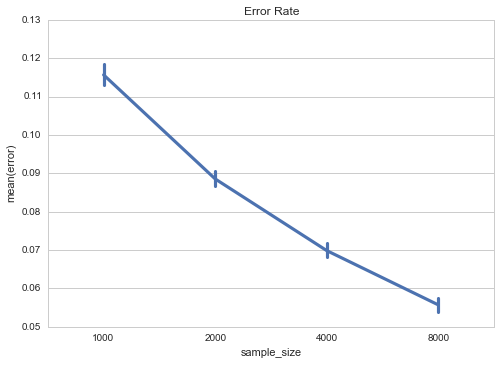
\includegraphics[scale=.5]{images/nn_error_rate}	
\end{center}


\section{Problem 2}
\paragraph{(a)} The formula for the MLE of the parameter $\mu_{y,j}$ is:
$$ x_j\log(\mu_j) + (1-x_j)\log(1-\mu_j) $$

\paragraph{(b)} The two functions used to answer this question can be found in the file problem2.py.  The first, named 'fit', takes takes two and one keyword argument.  The first positional argument X is the matrix of training features, and the second Y is the vector of labels.  The keyword argument 'laplace' takes a boolean value and determines whether or not the parameters use Laplace smoothing.  The function returns a matrix of parameters.  The second function, named 'predict', takes three positional arguments: 'params', the matrix of parameter vectors for each class, 'testdata', the matrix of test vectors to classify, and 'priors' the vector of class priors to use in computing the posteriors.  It returns a vector of predicted classes for each test document.

\paragraph{} Training the classifier yielded the following error rates on the training and testing datasets:

\begin{center}
\begin{tabular}{  c  c } 
Training Error & Testing Error \\
0.21705 & 0.37868 \\ 
\end{tabular}
\end{center}

\paragraph{(c)} The top twenty words for for each category were

\section{Problem 3}\label{previous work}
\paragraph{(a)}

\paragraph{(b)}

\section{Problem 4}\label{results}
\paragraph{(a)} The probability that two randomly selected balls have different colors is one minus the probability that any two similarly colored balls are selected. Since the probability of selecting two balls of the same color simultaneously is the $\big(\frac{n_{color}}{100}\big)^2$, the probability of choosing two similarly colored balls is the probability of selecting two of any of the colors, which is just the sum of the probabilities of any one of the colors. The probability of not getting any two colors is the complement of that, or:

$$ P(different) = 1 - \frac{n_r^2 + n_o^2 + n_y^2 + n_g^2 + n_b^2}{100^2}  $$

\paragraph{(b)} To maximize the probability that two different colors were chosen, I'd ensure that there were equal numbers of each color ball in the urn. More precisely, to maximize $$ P(different) = 1 - \frac{n_r^2 + n_o^2 + n_y^2 + n_g^2 + n_b^2}{100^2}  $$ subject to the constraint that $n_r + n_o + n_y + n_g + n_b = 100 $, I would use the Lagrangian Multiplier.

\end{document}
  